\chapter{膨張するニュートン宇宙}

\lectureoverview{現代宇宙論は、宇宙そのものを一つの物理系として扱うことから始まる。大規模な等方性と一様性を出発点として、共動格子を導入し、その運動を単一のスケール因子\(a(t)\)に符号化する。次にニュートンの球殻定理により、重力多体問題は\(a(t)\)に関する方程式へと変わる。エネルギー保存則は、再収縮する宇宙、臨界宇宙、永遠に膨張する宇宙を区別し、臨界物質優勢の場合から最初のフリードマン方程式と法則\(a(t)\propto t^{2/3}\)が得られる。}

\section{宇宙論が物理学になったとき}

宇宙論は学問としては古いが、定量的な宇宙論は若い。ここでの目的のためには、ギリシア人から始める必要はない。有用な歴史的出発点は、20世紀の第2四半期におけるハッブルによる宇宙膨張の発見、そして後に、およそ3ケルビンのマイクロ波背景放射が高温初期宇宙の名残であると認識されたことである。

測定が精密になる前は、天文学の多くは必然的に博物学に似ていた。珍しい恒星を見つけ、特異な銀河を分類し、測定できるものを測定し、天体のカタログを組み立てた。それらの天体は確かに物理系であり、角運動量を持ち、化学元素を含み、力学に従っていた。決定的な変化は、\emph{宇宙全体}を一つの物理系として扱い、観測と突き合わせるのに十分正確な方程式によって支配されるものとみなしたことである。

それがここでの主題である。われわれは宇宙の内容を列挙するだけではなく、その変数、その運動、その力学法則を問う。方程式は宇宙論の後に付け加えられる装飾ではない。それらは宇宙を物理学の問題にする手段である。

歴史的には、膨張する宇宙は一般相対性理論の言葉で理解された。しかし論理的には、最初の議論の多くはニュートン的である。正しい大規模運動を推測していた17世紀の物理学者なら、驚くほど良いモデルを導けたであろう。ニュートンから始める要点は、相対性理論を置き換えることではなく、相対性理論が後に幾何学的に再編成する力学を明らかにすることである。

\section{等方性、一様性、宇宙原理}

第一歩は観測的である。十分大きなスケールでは、宇宙は近似的に\emph{等方的}である。すなわち、天球の領域で平均し、天の川の前景を越えて見れば、どの方向にもほぼ同じに見える。これは厳密な一様性の主張ではない。近くの恒星を直接見ることは、空の領域を見ることとは異なり、物質の分布には実際の構造が含まれている。等方性は平均化された大規模な主張である。

一様性は別の主張である。それは、平均化された宇宙が場所ごとに同じであることを述べている。何銀河も離れた観測者も、同じ大規模平均の後には、われわれが見るのとほぼ同じ種類の宇宙を見るはずである。

第一近似では、銀河は単に質点として扱ってよい。可視宇宙にはおよそ
\begin{equation}
N_{\rm gal}\sim 10^{11}
\end{equation}
個の銀河があり、それぞれが桁で\(10^{11}\)個の恒星を持つ。これでおよそ\(10^{22}\)個の恒星が得られる。恒星あたり10個の惑星を意図的に粗い桁の推定として用いれば、\(10^{23}\)個の惑星に達し、面白いことに惑星1モルに近い。この数値推定は力学の一部ではないが、理想化される系のスケールを定める。

\begin{classroomqa}
\classquestion{観測可能な宇宙の中には、桁で言えば銀河がいくつあるか。}
\lecturerresponse{およそ一千億個、すなわち\(10^{11}\)である。銀河あたりおよそ\(10^{11}\)個の恒星があるとすれば、可視宇宙にはおよそ\(10^{22}\)個の恒星が存在することになる。以下の計算では各銀河を単一の質点で置き換えるが、これらは覚えておくと有用な規模の見積もりである。\lecturetimestamp{00:06:08--00:07:05}}
\end{classroomqa}

なぜわれわれの周りの等方性が一様性を示唆するのか。\emph{一様でない}等方的分布を想像してみよう。その密度は、方向に依存しないままでわれわれからの距離とともに変化しなければならない。事実上、われわれの位置を中心とする同心殻の模様を形成することになる。共通の中心からずれた観測者はもはや等方性を見ないであろう。したがって二つの可能性がある。
\begin{enumerate}
\item われわれが、宇宙がその周りに配置された特別な中心を占めている。または
\item 大規模分布が近似的に一様であり、どの占められた点も特別ではない。
\end{enumerate}
第二の可能性が経済的である。等方性と、われわれ自身に特権的な宇宙的位置を認めないこととを合わせると、一様性が導かれる。

\begin{classroomqa}
\classquestion{等方的だが一様でない分布はどのような形をとりうるか。}
\lecturerresponse{その変化は我々からの距離のみに依存し、我々の位置を中心とする殻状のパターンを生じうる。観測者をその中心から遠ざければ、パターンはもはや等方的でなくなる。我々の位置が特別でない限り、等方性はしたがって一様性を指し示す。\lecturetimestamp{00:07:06--00:08:54}}
\end{classroomqa}

この複合的な仮定は\emph{宇宙原理}と呼ばれる。十分に大きなスケールでは、宇宙は空間的に一様かつ等方である。これを原理と呼んでも証明にはならない。歴史的に、宇宙論者たちは観測がそれを強く正当化する前にこの仮定を採用した。その地位は経験的成功に由来する。

一様性もまた厳密ではない。銀河は銀河団や超銀河団を形成しており、可視天球の非常に大きな割合にわたって広がる構造についても長く議論されてきた。適切な主張は、平均領域が十分に大きければ、すなわちこの入門的な議論では数億光年からおよそ十億光年程度---であれば、揺らぎは平均化されて消えるというものである。そのスケールは観測によって精密化されるかもしれない。方法は、局所的な構造が記述を支配しなくなるまで粗視化することである。

\begin{classroomqa}
\audiencequestion{宇宙マイクロ波背景放射の一様性は宇宙原理の証拠を与えるか。}
\lecturerresponse{はい。宇宙原理はそれを支持する強い観測的根拠が存在する前に提唱されたが、後にマイクロ波背景放射は原始宇宙が極めて滑らかであったことを示した。銀河や銀河団はその滑らかな状態からの小さなずれから成長したのであり、それについての大規模な証拠を消し去るものではない。\lecturetimestamp{00:10:53--00:11:43}}
\end{classroomqa}

\section{銀河とともに動く格子}

観測的な近似を選んだなら、次に変数を選ばなければならない。「物理学の問題を定式化する第一歩は何か」という問いに対するある教室での答えは、変数を知ることである。伝統的な答えは、鉛筆を尖らせることである。ここでは、重要な変数は座標をうまく選ぶことによって見出される。

\(x,y,z\)というラベルを担う三次元の格子を想像せよ。これらのラベルはメートルで測った距離である必要はない。それらは座標の数である。小さな固有運動が平均化されて消えた後、すべての銀河が固定された格子点にとどまるように格子を選ぶ。そのとき銀河は\emph{共動}である。

そのような選択は、銀河がランダムに運動するならば役に立たないであろう。観測はむしろ、首尾一貫した大規模な運動を明らかにする。隣接する格子セルは膨張または収縮しうるが、同じ膨張または収縮がどこでも起こる。したがって、すべての物理的距離は、共通の時間依存スケールに固定された座標間隔を掛けたものとして書くことができる。

二つの銀河\(A\)と\(B\)について、
\begin{equation}
\begin{aligned}
d_{AB}(t)&=a(t)\,\Delta\chi_{AB},\\
\Delta\chi_{AB}
&=\sqrt{(x_A-x_B)^2+(y_A-y_B)^2+(z_A-z_B)^2}.
\end{aligned}
\label{eq:c01-physical-distance}
\end{equation}
それらが\(x\)座標のみで異なるならば、これは
\begin{equation}
d_{AB}(t)=a(t)\,\Delta x_{AB}.
\end{equation}
に帰着する。関数\(a(t)\)は\emph{スケール因子}である。その絶対的な規格化は慣習的である。すべての共動座標を定数倍し、\(a\)を同じ定数で割っても、物理的距離は変わらない。\(a(t_2)/a(t_1)\)のような比や、\(a\)で割った導関数が物理的な情報を担う。

式~\eqref{eq:c01-physical-distance}を微分せよ。共動間隔は固定されているので、
\begin{equation}
v_{AB}=\dot a\sqrt{(\Delta x)^2+(\Delta y)^2+(\Delta z)^2}.
\end{equation}
物理的距離で割ると
\begin{equation}
\frac{v_{AB}}{d_{AB}}=\frac{\dot a}{a}\equiv H(t),
\label{eq:c01-hubble-parameter}
\end{equation}
すなわち
\begin{equation}
\boxed{v_{AB}=H(t)d_{AB}.}
\label{eq:c01-hubble-law}
\end{equation}
となる。これは理想的な一様流におけるハッブルの法則である。

「ハッブル定数」という名は誤解を招きうる。ある宇宙時刻においては、\(H\)の同じ値が一様模型のあらゆる場所に当てはまるが、\(H(t)\)は一般に時間とともに変化する。空間的な普遍性は時間的な不変性ではない。

\begin{classroomqa}
\audiencequestion{すべての距離を一つの共通の\(a(t)\)に固定された座標間隔を掛けたものとして書くことによって、我々はすでにハッブルの法則を仮定してしまったのだろうか。}
\lecturerresponse{その仮定は確かにハッブルの観測に動機づけられている。首尾一貫した後退の証拠がなければ推測されなかったであろう。その価値は、その証拠を整理することにある。すべての銀河に独立な速度を割り当てる代わりに、単一の膨張する格子を記述する。ひとたびその記述を採用すれば、比例関係\(v=Hd\)は微分によって従う。\lecturetimestamp{00:24:20--00:25:33}}
\end{classroomqa}

同じ運動は二通りの言葉で記述できる。銀河は空間の中を互いに離れていくと言ってもよいし、銀河は固定された共動位置にとどまり、格子---、したがってそれらの間の物理的空間---が膨張すると言ってもよい。この段階では、これらは同じ数学に対する二つの座標記述である。一般相対性理論は膨張する空間という言葉を特に自然なものにするであろうが、どの時刻においても同じ物理的間隔を割り当てる二つの記述を区別できる観測は存在しない。

\section{共動セルにおける質量の帳簿付け}

重力を導入する前に、質量を追跡しておこう。座標体積
\begin{equation}
\Delta V_{\rm com}=\Delta x\,\Delta y\,\Delta z.
\end{equation}
をもつ小さな座標セルを考える。ただし、局所的な揺らぎを平均できるように、多数の銀河を含むのに十分な大きさでなければならない。\(\nu\) を単位共動座標体積あたりの質量とする。セル内の質量は
\begin{equation}
\Delta M=\nu\,\Delta x\,\Delta y\,\Delta z.
\label{eq:c01-comoving-mass}
\end{equation}
である。セルは物質とともに動くので、理想的な流れでは銀河がその境界を横切ることはなく、\(\Delta M\) は一定である。

各物理的辺は、対応する座標的辺より因子 \(a(t)\) だけ長い。したがって物理体積は
\begin{equation}
\Delta V_{\rm phys}=a^3(t)\,\Delta x\,\Delta y\,\Delta z.
\end{equation}
である。物理的質量密度は
\begin{equation}
\boxed{\rho(t)=\frac{\Delta M}{\Delta V_{\rm phys}}=\frac{\nu}{a^3(t)}.}
\label{eq:c01-density-dilution}
\end{equation}
である。膨張は無圧力物質を \(a^{-3}\) として希薄化し、収縮は同じ法則でそれを濃縮する。

ここまでは、動的なことは何も仮定していない。ユークリッド幾何学、運動学的な仮定、そして共動セルにおける質量保存を用いてきた。ここで重力が入ってくる。

\section{ここでニュートンが登場する}

無限に一様な物質分布は、一方からの引力が他方からの引力によって打ち消されるため静止し続けるはずだ、という誘惑的ながら誤った描像がある。欠陥は、この非形式的な打ち消しが相対加速度に対する整合的な方程式を与えないことにある。ニュートンの球殻定理が、力の正しい整理を与える。

任意の銀河を原点 \(O\) として選び、固定された共動半径
\begin{equation}
R=\sqrt{x^2+y^2+z^2}.
\end{equation}
にある銀河 \(A\) を考える。その物理半径、動径速度、動径加速度は
\begin{equation}
d=aR,
\qquad
\dot d=\dot a R,
\qquad
\ddot d=\ddot a R.
\label{eq:c01-radial-kinematics}
\end{equation}
である。

\begin{figure}[ht]
\centering
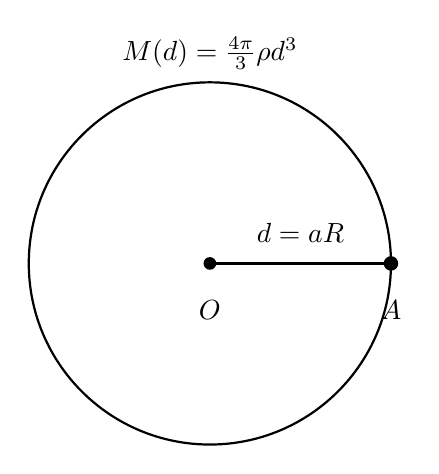
\begin{tikzpicture}[scale=1.15]
\draw[thick] (0,0) circle (2);
\fill (0,0) circle (0.07);
\fill (2,0) circle (0.08);
\draw[thick] (0,0) -- (2,0);
\draw (1,0.12) node[above] {\(d=aR\)};
\draw (0,-0.3) node[below] {\(O\)};
\draw (2,-0.3) node[below] {\(A\)};
\draw (0,2.32) node {\(M(d)=\frac{4\pi}{3}\rho d^3\)};
\end{tikzpicture}
\caption{ニュートン的還元。銀河 \(A\) の加速度に対して、外側の球殻は打ち消し合い、半径 \(d\) の内側の質量は \(O\) に集中しているかのように作用する。}
\label{fig:c01-newton-sphere}
\end{figure}

球対称な質量分布に対して、\(A\) を通る球の外側の物質からの正味の力は消える。内側の物質は中心に集中しているかのように作用する。囲まれた質量は
\begin{equation}
M(d)=\frac{4\pi}{3}\rho d^3.
\label{eq:c01-enclosed-mass}
\end{equation}
である。するとニュートンの逆二乗法則が \(A\) の加速度を与える：
\begin{equation}
\ddot d=-\frac{GM(d)}{d^2}.
\end{equation}
式~\eqref{eq:c01-radial-kinematics}を用いると、
\begin{align}
\ddot a R
&=-\frac{G}{d^2}\left(\frac{4\pi}{3}\rho d^3\right) \\
&=-\frac{4\pi G}{3}\rho d \\
&=-\frac{4\pi G}{3}\rho aR.
\end{align}
共動半径が打ち消され、
\begin{equation}
\boxed{\frac{\ddot a}{a}=-\frac{4\pi G}{3}\rho.}
\label{eq:c01-acceleration}
\end{equation}
が残る。この打ち消しが整合性の検査である。すべての共動銀河は、\(R\) によらず、同じスケール因子に対して同じ方程式に従う。

式~\eqref{eq:c01-density-dilution}を代入すると、等価な形のいずれかが得られる：
\begin{equation}
\frac{\ddot a}{a}=-\frac{4\pi G\nu}{3a^3},
\qquad
\ddot a=-\frac{4\pi G\nu}{3a^2}.
\label{eq:c01-acceleration-nu}
\end{equation}
第一の形は分数加速度を示し、第二の形は \(\ddot a\) を分離する。\(a\) を左辺に保つのは慣習であり、物理の変更ではない。

\begin{classroomqa}
\audiencequestion{原点は任意であったが、計算におけるすべての力はそこを向いている。原点を別に選ぶと、どうして同じ宇宙が得られるのか。}
\lecturerresponse{この方程式は相対運動に関するものである。他の任意の銀河のまわりで計算を繰り返しても、一様性により囲まれた質量が物理半径のみに依存するため、同じ方程式が得られる。別の銀河に付随する加速系へ変換しつつ、力を第一の原点を基準として保持するならば、対応する慣性力もまた含めなければならない。中心静止系を選ぶことは、その余分な帳簿付けを避けるだけのことである。不変な結果は式~\eqref{eq:c01-acceleration}であり、特別な中心ではない。\lecturetimestamp{00:43:56--00:46:58}}
\end{classroomqa}

\begin{classroomqa}
\audiencequestion{共動質量密度 \(\nu\) が場所ごとに変化するならば、この結果は生き残るだろうか。}
\lecturerresponse{この一関数の形では生き残らない。きれいな打ち消しは、\(M\propto d^3\) がどこでも同じ比例関係をもつことに依存している。もし \(\nu\) が平均化のスケールを越えて有意に変化するならば、異なる領域は異なる局所的な動力学を必要とし、単一の一様なスケール因子はもはやそれらを記述しないだろう。一様性が本質的な役割を果たしている。\lecturetimestamp{00:47:05--00:47:51}}
\end{classroomqa}

\begin{classroomqa}
\audiencequestion{なぜ因子 \(a\) を右辺に移さずに \(\ddot a/a\) と書くのか。}
\lecturerresponse{どちらの形も正しい。宇宙論では慣習的に分数加速度 \(\ddot a/a\) を書く。それは、分数膨張率 \(H=\dot a/a\) と直接比較できるからでもある。\(a\) を掛け合わせると同一の微分方程式が得られる。\lecturetimestamp{00:50:36--00:51:29}}
\end{classroomqa}

式~\eqref{eq:c01-acceleration}は、通常の物質で満たされた静的で一様なニュートン宇宙を直ちに排除する。静的なスケール因子では \(\ddot a=0\) となるが、正の密度は右辺を負にする。これは、宇宙が膨張しているか収縮しているかをまだ教えては\emph{いない}。それは加速度の符号だけを教える。

\section{負の加速度は収縮ではない}

速度と加速度の区別は初等的だが決定的である。アウトバーンを前進するフェラーリは正の速度を持ちながら、負の加速度で制動することができる。同様に、宇宙は
\begin{equation}
\dot a>0,
\qquad
\ddot a<0:
\end{equation}
膨張しているが、膨張は減速していることがありうる。

運動が最終的に反転するかどうかを決めるには、宇宙論的問題を地球の重力場中を半径方向に運動する試験粒子と比較せよ。ここで\(x\)は中心質量\(M\)からの粒子の物理的距離を表すものとし、先の共動座標とは無関係である。ニュートンの方程式は
\begin{equation}
\ddot x=-\frac{GM}{x^2}.
\label{eq:c01-particle-force}
\end{equation}
加速度は常に内向きである。外側へ投げられた粒子はそれでも長い間、あるいは永遠に外側へ進み続けるかもしれない。すでに内側へ運動している粒子はますます負に大きい速度を得る。力の法則だけではどちらの運動が起こるか決まらない。初期条件が決めるのである。

\begin{classroomqa}
\audiencequestion{\(\ddot a<0\)は宇宙が収縮していることを意味するのか。}
\lecturerresponse{いいえ。収縮とは\(\dot a<0\)を意味する。負の\(\ddot a\)は\(\dot a\)が時間とともに減少することを意味するにすぎない。もし\(\dot a\)が正で始まれば、重力は膨張を減速させる。それがゼロに達するかどうかは初期の膨張速度に依存し、ちょうど外側へ運動する発射体の運命が脱出速度を下回るか上回るかに依存するのと同様である。\lecturetimestamp{00:51:30--00:56:18}}
\end{classroomqa}

\begin{figure}[ht]
\centering
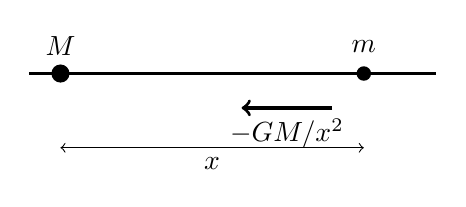
\begin{tikzpicture}[scale=1.15]
\fill (0,0) circle (0.1);
\draw (0,0.3) node {\(M\)};
\draw[thick] (-0.35,0) -- (4.15,0);
\fill (3.35,0) circle (0.08);
\draw (3.35,0.3) node {\(m\)};
\draw[->,very thick] (3.0,-0.38) -- (2.0,-0.38)
  node[midway,below] {\(-GM/x^2\)};
\draw[<->] (0,-0.82) -- (3.35,-0.82)
  node[midway,below] {\(x\)};
\end{tikzpicture}
\caption{加速度の符号を運動の方向と運命から分離するために用いられた半径方向の一粒子問題。}
\label{fig:c01-particle-sketch}
\end{figure}

エネルギーは選択肢を透明にする。保存される力学的エネルギーは
\begin{equation}
E=\frac12 m\dot x^{\,2}-\frac{GMm}{x}.
\label{eq:c01-particle-energy}
\end{equation}
ポテンシャルエネルギーは\(1/x\)に比例し、\(1/x^2\)ではない。\(-GMm/x\)を微分すると逆二乗の力が生じる。

\begin{figure}[ht]
\centering
\includegraphics[width=0.82\textwidth]{lecture_01_figure_02.png}
\caption{エネルギー論の冒頭における板書：重力ポテンシャルエネルギーが復元される直前の、運動する試験質量とその運動項。}
\lectureframe{00:58:57}
\end{figure}

もし\(E<0\)ならば、外側へ運動する粒子は無限遠に到達できない。そこではポテンシャルエネルギーがゼロに近づき、運動エネルギーは非負である。それは有限の\(x\)で停止し、戻らなければならない。もし\(E>0\)ならば、それは停止できない。なぜなら転回点では運動エネルギーがゼロになり、残りのポテンシャルエネルギーが負になるが、これは正の\(E\)の保存に矛盾するからである。境界は
\begin{equation}
E=0,
\end{equation}
であり、これが脱出速度を定義する：
\begin{equation}
\frac12 m v_{\rm esc}^2-\frac{GMm}{x}=0,
\qquad
\boxed{v_{\rm esc}^2=\frac{2GM}{x}.}
\label{eq:c01-escape-velocity}
\end{equation}

\begin{figure}[ht]
\centering
\includegraphics[width=0.88\textwidth]{lecture_01_figure_03.png}
\caption{板書上で形を成しつつあるゼロエネルギーの境界。先の宇宙論的加速度方程式は左側に枠囲みで残り、半径方向の脱出問題が右側で展開されている。}
\lectureframe{01:01:37}
\end{figure}

ちょうど脱出速度においては、粒子は無限に減速する。その速さは\(x\to\infty\)としてのみゼロに近づき、有限の転回点には決して到達しない。この境界的な場合は最も単純な宇宙論的モデルとなるであろう。

\section{宇宙論的エネルギー方程式}

固定された共動半径\(R\)にある銀河に戻る。球殻定理により、その半径方向の運動は、その共動球が囲む質量に等しい点質量の外側を運動する粒子の運動と同一である。

\begin{figure}[ht]
\centering
\includegraphics[width=0.82\textwidth]{lecture_01_figure_04.png}
\caption{一粒子エネルギー論を宇宙論に戻す際に用いられた逆二乗の力と半径方向粒子のスケッチ。}
\lectureframe{01:04:14}
\end{figure}

囲まれた質量は物理的な球が膨張しても増加しない。球は共動的であり、常に同じ銀河を含む：
\begin{align}
M
&=\frac{4\pi}{3}\rho(aR)^3 \\
&=\frac{4\pi}{3}\frac{\nu}{a^3}a^3R^3 \\
&=\frac{4\pi}{3}\nu R^3.
\label{eq:c01-fixed-enclosed-mass}
\end{align}
最初の表式は密度の希薄化が含まれるまでは時間依存に見える。\(a^3\)の因子は相殺する。

\begin{classroomqa}
\audiencequestion{球が膨張するにつれて、それはより多くの質量を囲むのか。}
\lecturerresponse{いいえ。その物理的半径は成長するが、その共動境界は銀河とともに動く。理想的な均質流れでは境界を横切る物質はなく、方程式~\eqref{eq:c01-fixed-enclosed-mass}はその相殺を明示的に示している。\lecturetimestamp{01:04:37--01:05:20}}
\end{classroomqa}

銀河の物理的速度は\(\dot d=\dot a R\)であり、選ばれた原点からの距離は\(d=aR\)である。したがってその保存されたニュートン的エネルギーは
\begin{equation}
\boxed{
E=\frac12 m\dot a^{\,2}R^2-\frac{GMm}{aR}.
}
\label{eq:c01-cosmological-energy}
\end{equation}

\begin{figure}[ht]
\centering
\includegraphics[width=0.82\textwidth]{lecture_01_figure_05.png}
\caption{板書上の宇宙論的運動項とポテンシャル項。方程式~\eqref{eq:c01-cosmological-energy}における完全な分母\(aR\)は物理的半径と付随する導出から従う。}
\lectureframe{01:06:12}
\end{figure}

三つの粒子エネルギーの場合が、三つの宇宙論的な場合になる：
\begin{description}[style=nextline]
\item[\(E<0\)：] 初期膨張は脱出速度より小さい；\(a(t)\) は最大値に達し、宇宙は再収縮する。
\item[\(E=0\)：] 宇宙はちょうど臨界であり、膨張は永遠に減速し、速度零に漸近的にのみ近づく。
\item[\(E>0\)：] 初期膨張は脱出速度より大きい；ニュートン模型では宇宙は永遠に膨張し、漸近的な後退速度は非零である。
\end{description}

まず縁の場合 \(E=0\) から始める。方程式~\eqref{eq:c01-cosmological-energy}を零と置き、\(m\)を消去し、\(a^2R^2/2\)で割ると
\begin{align}
\frac12\dot a^{\,2}R^2&=\frac{GM}{aR}, \\
\left(\frac{\dot a}{a}\right)^2&=\frac{2GM}{a^3R^3}.
\label{eq:c01-energy-intermediate}
\end{align}
が得られる。
\begin{equation}
\rho=\frac{M}{(4\pi/3)a^3R^3},
\end{equation}
であるから、方程式~\eqref{eq:c01-energy-intermediate}は
\begin{equation}
\boxed{
H^2=\left(\frac{\dot a}{a}\right)^2=\frac{8\pi G}{3}\rho.
}
\label{eq:c01-first-friedmann}
\end{equation}
となる。これは、空間的に平坦で物質のみからなり、宇宙定数が零の宇宙に対する第一フリードマン方程式であり、ここではニュートン的なエネルギー保存から得られた。

\begin{classroomqa}
\classquestion{ちょうど脱出速度で打ち出された粒子はどうなるか。}
\lecturerresponse{それは反転することなく減速する。その速度は無限遠においてのみ零に近づく。零エネルギーの宇宙も同じように振る舞う：\(H\)は減少するが、\(\dot a\)は正のままであり、有限時間での転回は起こらない。\lecturetimestamp{01:10:45--01:12:10}}
\end{classroomqa}

因子\(4\pi/3\)と\(8\pi G/3\)は恣意的な装飾ではない。\(4\pi/3\)は球の体積であり、因子2は運動エネルギーから来る。一般相対性理論では同じ\(8\pi G\)がアインシュタインの場の方程式に現れ、その時間-時間成分が相対論的フリードマン方程式を導く。この一致は偶然ではないが、現在の導出にはまだ圧力、幾何学としての空間曲率、宇宙定数が含まれていない。

\section{臨界物質支配解}

密度則\(\rho=\nu/a^3\)を方程式~\eqref{eq:c01-first-friedmann}に用いる：
\begin{equation}
\left(\frac{\dot a}{a}\right)^2=\frac{8\pi G\nu}{3a^3}.
\label{eq:c01-matter-friedmann}
\end{equation}
定数\(\nu\)は共動座標の恣意的な規格化に依存する。時間依存性を明らかにするために、
\begin{equation}
K\equiv\frac{8\pi G\nu}{3}>0.
\end{equation}
と定義する。すると
\begin{equation}
\dot a^{\,2}=\frac{K}{a}.
\label{eq:c01-normalized-friedmann}
\end{equation}

\begin{figure}[ht]
\centering
\includegraphics[width=0.76\textwidth]{lecture_01_figure_06.png}
\caption{黒板に書かれた物質支配フリードマンスケーリング。まず定数を含む形で、次にスケール因子の本質的な逆冪を露わにした形で示されている。}
\lectureframe{01:14:44}
\end{figure}

方程式~\eqref{eq:c01-normalized-friedmann}の右辺は、任意の有限な正の\(a\)において正である。転回には\(\dot a=0\)が必要であるから、臨界宇宙は決して転回しない。その膨張は着実に疲れていくが、止まるほどに疲れることは決してない。

次に方程式を解く。直接変数を分離してもよい：
\begin{equation}
a^{1/2}\,da=\sqrt{K}\,dt,
\end{equation}
あるいは講義に従って冪則を試みてもよい：
\begin{equation}
a(t)=Ct^p.
\label{eq:c01-power-trial}
\end{equation}
すると
\begin{equation}
\frac{\dot a}{a}=\frac{p}{t},
\qquad
\frac{K}{a^3}=\frac{K}{C^3t^{3p}}.
\end{equation}
方程式~\eqref{eq:c01-matter-friedmann}への代入により
\begin{equation}
\frac{p^2}{t^2}=\frac{K}{C^3t^{3p}}.
\end{equation}
が得られる。冪と係数を一致させると
\begin{equation}
3p=2,
\qquad
C^3=\frac{K}{p^2}=\frac{9K}{4}.
\end{equation}
となる。したがって
\begin{equation}
\boxed{
a(t)=\left(\frac{3\sqrt K}{2}t\right)^{2/3}\propto t^{2/3}.
}
\label{eq:c01-two-thirds}
\end{equation}
時間の加法原点は、\(t=0\)において\(a=0\)となるように選ばれている。より一般には、\(t\)を\(t-t_0\)で置き換えてもよい。

スケール因子は永遠に増大するが、
\begin{equation}
\dot a\propto t^{-1/3}\longrightarrow0,
\qquad
H=\frac{2}{3t}\longrightarrow0.
\label{eq:c01-asymptotic-slope}
\end{equation}
そのグラフは常に増加し、常に下に凸である。\(a(t)\)自体が非有界であるため水平線には近づかないが、その傾きは零に近づく。

\begin{classroomqa}
\audiencequestion{\(t^{2/3}\)は、その試行形がたまたまうまくいったから見つかっただけなのか。別の試行形は別の零エネルギー解を与えうるか。}
\lecturerresponse{その試行形は、単に一つの可能性ではなく解そのものを同定する。一次の膨張枝の方程式\(\dot a=\sqrt{K/a}\)は、規格化と時間原点の選択を除いて一意的に\(a\propto(t-t_0)^{2/3}\)へと積分される。異なる全エネルギーは異なる微分方程式を与え、したがって異なる宇宙論的歴史を与える。\lecturetimestamp{01:27:07--01:27:43}}
\end{classroomqa}

\begin{classroomqa}
\audiencequestion{臨界曲線は最終的に水平になるのか。}
\lecturerresponse{その傾きは零に近づく：\(\dot a\propto t^{-1/3}\)。それでも任意の有限時間において正であるから、スケール因子は無限に増大し続ける。宇宙は静止に漸近的に近づくが、到達はしない。\lecturetimestamp{01:27:48--01:28:57}}
\end{classroomqa}

この単純な結果は歴史的に際立っている。ニュートンはこの導出に必要な力学と球殻定理を有しており、無限の重力を及ぼす宇宙についての問いを考察していたが、膨張模型を定式化しなかった。教室での議論では、宇宙の歴史に関する哲学的・神学的な信念が、彼にとってどのような問いが自然に思われるかに影響した可能性が示唆された。その歴史的な示唆は導出の一部ではなく、数学的な要点は、必要なニュートン的道具がすでに存在していたということだけである。

\begin{classroomqa}
\audiencequestion{このニュートン的な構成は無限宇宙を仮定しているのか。}
\lecturerresponse{それはユークリッド的で空間的に平坦なニュートン空間を仮定している。通常のニュートンモデルではその空間は無限に広がるため、共動銀河間の距離が時間とともに変化するとしても、モデルは空間的に無限である。曲がった有限な空間幾何は相対論的取り扱いに属する。\lecturetimestamp{01:22:12--01:22:55}}
\end{classroomqa}

\section{ゼロエネルギー模型を超えて}

ゼロエネルギーの場合は意図的な単純化であり、唯一のニュートン宇宙ではない。式~\eqref{eq:c01-cosmological-energy}で\(E\neq0\)を保つと
\begin{equation}
\left(\frac{\dot a}{a}\right)^2
=\frac{8\pi G}{3}\rho+\frac{2E}{mR^2a^2}.
\label{eq:c01-nonzero-energy}
\end{equation}
が得られる。一様性は、組み合わせ\(2E/(mR^2)\)がすべての代表的な共動球に対して同じであることを要求する。これを定数\(C_E\)と書くと、
\begin{equation}
H^2=\frac{8\pi G}{3}\rho+\frac{C_E}{a^2}.
\end{equation}
正の\(C_E\)は脱出エネルギーを超えることに対応し、負の\(C_E\)は転回を許す。相対論的表記では、このエネルギー項は空間曲率を通じて再解釈される。この関連は後の取り扱いに取っておく。

物質のみの三つの歴史はすべて、物質が支配的な間は負の加速度をもつ：
\begin{equation}
\ddot a=-\frac{4\pi G}{3}\rho a<0.
\end{equation}
再収縮する曲線は上昇し、\(\dot a=0\)に達してから下降する。臨界曲線\(t^{2/3}\)は傾きがゼロに近づきながら永遠に上昇する。正エネルギーの曲線もまた永遠に上昇し、線形成長に近づく。これらの場合についての暫定的な板書スケッチは講義中に訂正された。安定した結論は、最初のスケッチの細部すべてではなく、共通する下に凸な振る舞いである。

観測される宇宙はさらに多くを行う。その初期の物質支配膨張は減速する曲線でよく近似されるが、後期には曲線は上向きに曲がる：
\begin{equation}
\ddot a>0.
\end{equation}
通常の無圧力物質は式~\eqref{eq:c01-acceleration}においてその符号を生み出せない。追加の項が必要である。最も単純な現代モデルではそれは宇宙定数であり、より一般にはダークエネルギーと呼ばれる。本章では、ニュートン的な物質動力学をまず清潔に理解できるように、意図的にそれを省いている。

\begin{classroomqa}
\audiencequestion{フリードマン方程式の\(8\pi G\)はアインシュタインの場の方程式に現れる同じ因子か、また宇宙定数を含めたのか。}
\lecturerresponse{同じ重力の規格化が一般相対論にも現れ、時間-時間場の方程式は相対論的フリードマン方程式を再現する。ここでのモデルには宇宙定数は含まれない。それは物質支配宇宙であり、欠けている宇宙定数項はまさに後期の加速を説明しうる種類の項である。\lecturetimestamp{01:30:15--01:31:06}}
\end{classroomqa}

\section{平均流と局所的なずれ}

一様膨張は粗視化された記述である。それはすべての物体が近傍のあらゆる隣から遠ざかるように膨張するとは述べていない。重力的あるいはその他の理由で束縛された系はハッブル流から切り離されうる。たとえば天の川銀河とアンドロメダ銀河は、大規模な後退法則に従うのではなく、互いに近づいている。

個々の銀河の速度がハッブル流からずれることを、その\emph{特異速度}と呼ぶ。この用語は技術的なものであり、銀河に対する判断ではない。ハッブルの法則は、より大きな距離とより大きな体積で平均するほど良い近似となる。束縛された銀河、銀河団、あるいは局所的に過密な領域のスケールでは、局所的な力が背景膨張を支配しうる。

\begin{classroomqa}
\audiencequestion{宇宙が全体として膨張していても、いくつかの領域は収縮しうるか。}
\lecturerresponse{もちろんである。束縛された系や十分に高密度な揺らぎは平均膨張に従う必要はない。天の川銀河--アンドロメダ銀河系は身近な例である。宇宙論的な計算は、これらの特異運動や局所的な密度揺らぎが支配しないほど大きな体積で平均する。その結果得られる\(a(t)\)は背景を記述するのであり、すべての物体の対を記述するのではない。\lecturetimestamp{01:31:00--01:34:13}}
\end{classroomqa}

類推は普通の気体である。部屋の空気を一様と呼ぶことは、分子の揺らぎや密度の局所的な変動を否定しない。それは、十分に大きな領域での平均が安定していると言っているのである。宇宙の一様性も同じ論理的地位をもつが、はるかに大きなスケールにおいてである。平均よりわずかに高密度に生まれた領域は、膨張に抵抗し最終的に束縛構造へと崩壊するのに十分な自己重力をもちうる。

\begin{classroomqa}
\audiencequestion{銀河が空間の中を運動しているのか、それとも膨張する空間が銀河を互いに引き離して運んでいるのかを、観測によって決めることができるだろうか。}
\lecturerresponse{二つの記述がすべての対に同じ距離\(d_{AB}(t)\)を割り当てる場合には、できない。一方の記述では銀河は固定して見える座標背景の上を運動し、共動記述では銀河を凍結してスケール因子に変化を担わせる。両者は数学的に等価である。一般相対性理論は第二の言語をより自然にするが、この比較において別個の観測量を生み出すわけではない。\lecturetimestamp{01:34:14--01:34:59}}
\end{classroomqa}

\begin{classroomqa}
\audiencequestion{Ia型超新星の明るさ以外に、宇宙の加速を支持する独立の証拠はあるだろうか。}
\lecturerresponse{ある。この推論は観測のネットワーク、とりわけ超新星の測定と宇宙マイクロ波背景放射がどのように整合するかから導かれる。単一のデータが結論のすべてを担うのではなく、独立な宇宙論的測定の間の整合性が重要な点である。\lecturetimestamp{01:35:00--01:35:38}}
\end{classroomqa}

\section{確立されたこと}

議論は厳密な順序で進んできた。
\begin{enumerate}
\item 大規模な等方性と、特権的な中心の否定とから、一様性が動機づけられる。
\item 一様性は、一つのスケール因子\(a(t)\)をもつ共動格子を許す。
\item 物理的距離を微分するとハッブルの法則が得られる。
  \[
  H=\frac{\dot a}{a},
  \qquad
  v=Hd.
  \]
\item 共動セルにおける質量の保存から
  \[
  \rho=\frac{\nu}{a^3}.
  \]
\item ニュートンの球殻定理から加速度方程式
  \[
  \frac{\ddot a}{a}=-\frac{4\pi G}{3}\rho.
  \]
\item 保存されたエネルギーが、再収縮する膨張、臨界膨張、束縛されない膨張を分類する。
\item 全エネルギーがゼロのとき、
  \[
  H^2=\frac{8\pi G}{3}\rho,
  \qquad
  a(t)\propto t^{2/3}.
  \]
\end{enumerate}

これは完全なニュートン的物質支配模型であるが、まだ我々の宇宙の完全な記述ではない。それは初期の減速する論理を捉え、満たされた一様な宇宙がなぜ静的であり続けられないかを示し、脱出の縁にある臨界膨張を同定する。ゼロでないエネルギー、相対論的な空間幾何、圧力、放射、そして後期の加速を担う項は、なお付け加えられるべきものである。
